\documentclass[11pt,a4paper]{article}

\usepackage[top=2.54cm, bottom=2.54cm, left=2.54cm, right=2.54cm]{geometry}
\usepackage{fontspec}
\usepackage{amsmath, amssymb}
\usepackage{graphicx}
\usepackage{booktabs}
\usepackage{tabularx}
\usepackage{array}
\usepackage{enumitem}
\usepackage{caption}
\usepackage{cite}
\usepackage{xcolor}
\usepackage{fancyhdr}
\usepackage{titlesec}
\usepackage[colorlinks=true, linkcolor=blue!80!black, citecolor=blue!80!black, urlcolor=blue!80!black]{hyperref}

% Configure Fonts
\setmainfont{Times New Roman}
\newfontfamily\zhfont{SimSun}[AutoFakeBold=true]
\newfontfamily\zhheiti{SimHei}[AutoFakeBold=true]

% Enable automatic Chinese character line wrapping
\XeTeXlinebreaklocale "zh"
\XeTeXlinebreakskip = 0pt plus 1pt

% Chinese Font Size Helpers (zihao)
\newcommand{\zihao}[1]{%
  \ifcase#1\relax
    \fontsize{42pt}{48pt}\selectfont % 0
  \or
    \fontsize{26pt}{30pt}\selectfont % 1
  \or
    \fontsize{22pt}{26pt}\selectfont % 2
  \or
    \fontsize{16pt}{20pt}\selectfont % 3
  \or
    \fontsize{14pt}{18pt}\selectfont % 4
  \or
    \fontsize{10.5pt}{13pt}\selectfont % 5
  \else
    \fontsize{10.5pt}{13pt}\selectfont
  \fi
}

% Section title formatting
\titleformat{\section}{\large\bfseries}{\thesection}{1em}{}
\titleformat{\subsection}{\normalsize\bfseries}{\thesubsection}{1em}{}
\titleformat{\subsubsection}{\small\bfseries}{\thesubsubsection}{1em}{}
\titlespacing*{\section}{0pt}{10pt plus 2pt minus 2pt}{4pt plus 1pt minus 1pt}
\titlespacing*{\subsection}{0pt}{8pt plus 2pt minus 2pt}{3pt plus 1pt minus 1pt}

% Headers and Footers matching NPU template (-1-, -2-, etc.)
\pagestyle{fancy}
\fancyhf{}
\renewcommand{\headrulewidth}{0pt}
\cfoot{-\ \thepage\ -}

% Line spacing
\linespread{1.15}

\begin{document}

% Page 1: Cover
\begin{titlepage}
\thispagestyle{empty}

% Top right: Student ID Box
\begin{flushright}
\begin{tabular}{c@{\ }l}
{\zhfont 学号} & \\
Student No.: & \underline{\makebox[3.2cm][c]{\large 2025291043}}
\end{tabular}
\end{flushright}

\vspace{1.7cm}

% Large Title
\begin{center}
    {\fontspec{KaiTi}\zihao{2} 西北工业大学研究生学位论文选题报告表} \\[0.35cm]
    {\zihao{3} Northwestern Polytechnical University} \\[0.25cm]
    {\zihao{3} Graduate Degree Dissertation Title Selection Report Form}
\end{center}

\vspace{2.6cm}

% Form Table matching the NPU template exactly (strictly NO underlines below Chinese text)
\begin{center}
\large
\renewcommand{\arraystretch}{1.2}
\begin{tabular}{c l}
    \makebox[3.1cm][s]{{\zhfont 学}\hfill{\zhfont 院}} & \quad{\zhfont 计算机学院} \\
    \makebox[3.1cm][c]{School} & \underline{\makebox[8.5cm][l]{\quad School of Computer Science}} \\[0.15cm]
    
    \makebox[3.1cm][s]{{\zhfont 学}\hfill{\zhfont 科、}\hfill{\zhfont 专}\hfill{\zhfont 业}} & \quad{\zhfont 计算机科学与技术} \\
    \makebox[3.1cm][c]{Discipline / Specialty} & \underline{\makebox[8.5cm][l]{\quad Computer Science and Technology}} \\[0.15cm]
    
    \makebox[3.1cm][s]{{\zhfont 姓}\hfill{\zhfont 名}} & \quad{\zhfont 大雷} \\
    \makebox[3.1cm][c]{Name} & \underline{\makebox[8.5cm][l]{\quad DAULET ANEKESH}} \\[0.15cm]
    
    \makebox[3.1cm][s]{{\zhfont 学}\hfill{\zhfont 位}\hfill{\zhfont 级}\hfill{\zhfont 别}} & \quad{\zhfont 硕士} \\
    \makebox[3.1cm][c]{Degree} & \underline{\makebox[8.5cm][l]{\quad Master}} \\[0.15cm]
    
    \makebox[3.1cm][s]{{\zhfont 导}\hfill{\zhfont 师}} & \quad{\zhfont 郭斌} \\
    \makebox[3.1cm][c]{Supervisor} & \underline{\makebox[8.5cm][l]{\quad Prof. Bin Guo}} \\[0.15cm]
    
    \makebox[3.1cm][s]{{\zhfont 培}\hfill{\zhfont 养}\hfill{\zhfont 类}\hfill{\zhfont 别}} & \quad{\zhfont 留学研究生} \\
    \makebox[3.1cm][c]{Category} & \underline{\makebox[8.5cm][l]{\quad Overseas Postgraduates}} \\[0.15cm]
    
    \makebox[3.1cm][s]{{\zhfont 报}\hfill{\zhfont 告}\hfill{\zhfont 日}\hfill{\zhfont 期}} & \quad{\zhfont 2026年10月} \\
    \makebox[3.1cm][c]{Date of Report} & \underline{\makebox[8.5cm][l]{\quad October 2026}}
\end{tabular}
\end{center}

\vfill

% Bottom: Graduate School
\begin{center}
    {\fontspec{KaiTi}\zihao{3} 研\quad 究\quad 生\quad 院} \\[0.2cm]
    {\zihao{4} Graduate School}
\end{center}

\vspace{0.0cm}
\end{titlepage}


% Page -1-: Requirements
\clearpage
\setcounter{page}{1}
\begin{center}
    {\zhheiti\zihao{3}\bfseries 研究生学位论文选题报告的要求}
\end{center}

\vspace{0.2cm}

\begin{enumerate}[leftmargin=2.2em, itemsep=2pt, topsep=2pt, parsep=0pt]
    \item[{\zhfont 一、}] {\zhfont 硕士生的选题报告内容应包括文献综述、选题意义、研究内容、研究方案，论文工作量的估计、工作条件，预期达到的水平，存在的问题及拟采取的解决措施。}
    \item[{\zhfont 二、}] {\zhfont 博士生的选题报告内容应包括文献综述、选题背景及其意义、研究内容、研究特色、工作难点、预期成果及其可能的创新点。}
    \item[{\zhfont 三、}] {\zhfont 选题报告会应以学术活动的方式公开进行。}
    \item[{\zhfont 四、}] {\zhfont 正式开题之前，研究生应在广泛阅读中、外文资料的基础上，深入了解拟选课题的国内外研究动态，把握所选课题的目的、意义和预期结果，明确课题工作的设想、方法和研究路径。}
    \item[{\zhfont 五、}] {\zhfont 研究生在规定的时间内，写出选题报告初稿，经指导教师审阅同意后，由指导教师安排选题报告时间。选题报告未通过者，重新开题，若第二次选题报告仍通不过者，则按有关规定终止学籍。}
    \item[{\zhfont 六、}] {\zhfont 选题报告不能按期完成者，应及时向研究生院培养处提出延期申请。}
    \item[{\zhfont 七、}] {\zhfont 本表可以打印或用钢笔认真填写，若不够填写时，可另加附页。}
\end{enumerate}

\vspace{0.4cm}

\begin{center}
    {\zihao{3}\textbf{Requirements for the Dissertation Title Selection Report}}
\end{center}

\vspace{0.2cm}

\begin{enumerate}[label={\arabic*.}, leftmargin=2.2em, itemsep=2pt, topsep=2pt, parsep=0pt]
    \item The Dissertation Title Selection Report for Master Degrees should include the Literature Review, the Meaning of the Title Selection, the Research Contents, the Research Plan, Workload Estimation, Working Conditions, the Goal to Achieve, Problems Existing as well as the Measures to Take.
    \item The Dissertation Title Selection Report for PhD Degrees should include Literature Review, Background and Meaning of the Selection, Research Contents, Characteristics of the Research, Difficulties, Goals to Achieve and possible Innovations.
    \item The Report should be made in public as academic activities.
    \item Before starting the title, graduates should, based on the extensive reading through the literature both in Chinese and in foreign languages, have a deep command of the research tendency home and abroad. They must have a clear mind of the aim, meaning and foreseen results, research assumption, methods and approaches.
    \item Graduates should finish the draft report within the required time, and then the supervisor after having checked the report, organizes time to make the report. Those who fail to pass the report have to reopen a title. If it can not be passed for a second time, the studentship will be stopped.
    \item Those who can not finish the report on time should forward application to the Graduate School to extend the duration.
    \item The form should be filled out in pen or printed. If the pages are not enough, extra pages can be attached.
\end{enumerate}


% Page -2- onwards: Main Report
\clearpage
\newpage

% Table Header Box matching Page -2- of NPU form
\noindent
\begin{tabularx}{\textwidth}{|p{3.0cm}|X|X|X|X|}
\hline
\centering \textbf{\zhfont 论文题目} \newline \textbf{Dissertation Title} & 
\multicolumn{4}{p{\dimexpr\textwidth-3.0cm-4\tabcolsep-3\arrayrulewidth\relax}|}{\raggedright \textbf{Morphologically-Grounded AI-Generated Text Detection and Factual Verification for Low-Resource Agglutinative Languages: A Comprehensive Framework for Kazakh}} \\
\hline
\centering \textbf{\zhfont 论文类型} \newline {\zhfont\footnotesize (在有关项目下作记号$\surd$)} \newline \textbf{Dissertation Type} \newline {\footnotesize (Put a tick $\surd$ under relevant item)} &
\centering {\zhfont 基础研究} \newline {\footnotesize Fundamental Research} &
\centering {\zhfont 应用研究} \newline {\footnotesize Application Research} \newline \textbf{\Large $\surd$} &
\centering {\zhfont 工程技术} \newline {\footnotesize Engineering Technology} &
\centering {\zhfont 跨学科研究} \newline {\footnotesize Research Cross Discipline} \tabularnewline
\hline
\multicolumn{5}{|p{\dimexpr\textwidth-2\tabcolsep-2\arrayrulewidth\relax}|}{
{\zhfont 研究生在进行选题报告、听取意见后，整理成文（不少于 3500 字）。} \newline
\textbf{After the report and comments, make the records up to an article. (no less than 3500 words)}
} \\
\hline
\end{tabularx}

\vspace{0.6cm}

\section{Research Background}
\label{sec:background}

\subsection{Relevance and Context}
\label{sec:relevance_and_context}

The rapid evolution and widespread deployment of autoregressive Large Language Models (LLMs)---such as OpenAI's GPT-4, Meta's LLaMA-3, DeepSeek-R1, and multilingual open foundation architectures including Cohere's Aya---have fundamentally transformed artificial intelligence, automated reasoning, and natural language communication \cite{vaswani2017attention, achiam2023gpt4, dubey2024llama3, guo2025deepseekr1, ustun-etal-2024-aya}. These foundation models demonstrate exceptional proficiency in generating syntactically coherent, stylistically diverse, and contextually fluent texts across numerous domain contexts. However, the universal accessibility of advanced generative models has simultaneously escalated severe risks concerning information integrity, epistemic credibility, and digital safety \cite{bender2021stochasticparrots, solaiman2019release}. Contemporary digital ecosystems face increasing exposure to synthetic text artifacts, ranging from automated disinformation campaigns and fraudulent consumer reviews to AI-assisted academic plagiarism and hallucinated pseudo-factual assertions delivered with unmerited confidence.

Consequently, establishing robust computational mechanisms for auditing digital text content has emerged as an imperative requirement for trustworthy artificial intelligence. Reliable information verification demands two foundational capabilities: (1) \textit{AI-generated text detection}, which identifies generative origin by discerning whether a candidate text was composed by a human or synthesized by an autoregressive neural network; and (2) \textit{automated fact verification}, which evaluates whether factual propositions are substantiated by reputable reference evidence.

While extensive research has advanced text auditing in high-resource, typologically analytic or mildly fusional languages such as English and Standard Mandarin, existing methods encounter fundamental performance bottlenecks when deployed in low-resource, morphologically complex agglutinative languages \cite{khurana2024subwords, togmanov-etal-2025-kazmmlu}. Languages of the Turkic family---exemplified by Kazakh, which serves as the official state language of Kazakhstan and is spoken by over 15 million people across Central Asia---possess typological structures that directly challenge standard deep learning assumptions. In agglutinative linguistic systems, lexical roots serve as anchors for extensive, sequential suffixation chains that encode negation, syntactic case relations, tense, evidentiality, possessive markers, and pragmatic moods within single polymorphemic words. A solitary verbal root can produce hundreds of distinct surface wordforms without introducing new lexical headwords.

The proliferation of multilingual generative models within Central Asian educational, administrative, and public communication ecosystems underscores an urgent sovereign need for language-native text verification infrastructure. Without specialized auditing tools tailored to the morphological properties of Kazakh, regional media environments remain acutely vulnerable to synthetic manipulation. Developing linguistically grounded detection and verification frameworks is therefore essential for ensuring information security and linguistic equity.

\subsection{Challenges of Existing AI Detection Systems}
\label{sec:challenges_existing}

Despite substantial progress in machine-generated text detection, contemporary detection paradigms exhibit critical vulnerabilities when applied to Kazakh and typologically similar agglutinative languages:

\begin{enumerate}[leftmargin=*, label=(\arabic*)]
    \item \textbf{Subword Tokenization Fragmentation:} Prevailing transformer architectures rely on statistical subword algorithms, such as Byte-Pair Encoding (BPE), WordPiece, or SentencePiece \cite{khurana2024subwords}. These algorithms are predominantly trained on high-resource multilingual corpora, optimizing vocabulary merge operations based purely on surface frequency rather than grammatical structure. In agglutinative languages, standard tokenizers aggressively partition polymorphemic words across arbitrary character boundaries, fragmenting functional affixes into meaningless byte sequences. As illustrated in Figure~\ref{fig:fst_fragmentation}, the Kazakh word \textit{мектебіміздегілерден} (``from those who are in our school'') contains a transparent grammatical sequence of root, possessive, locative, adjectivizer, plural, and ablative morphemes. Standard subword tokenizers partition this single word into disjoint subword fragments, obscuring both the root lemma and the inflectional markers. This fragmentation inflates effective sequence lengths, depletes transformer context windows, and attenuates gradient propagation during representation learning.
    
    \item \textbf{Absence of Morphological Priors and Linguistic Grounding:} Conventional neural detectors treat text as unconstrained surface token sequences, lacking explicit inductive biases regarding root-affix compositionality, vowel harmony (palatal and labial harmony), and morphotactic suffix ordering \cite{khoshhal2020kazakh, tyers2012free}. As a result, neural classifiers struggle to distinguish natural inflectional richness from synthetic generation artifacts, frequently misclassifying formal, highly inflected human prose as machine-generated text.
    
    \item \textbf{Severe Cross-Generator and Out-of-Domain Degradation:} Zero-shot probability curvature methods (such as DetectGPT \cite{mitchell2023detectgpt}, Binoculars \cite{hans2024binoculars}, and Fast-DetectGPT \cite{bao2024fastdetectgpt}) depend on surrogate language models to evaluate local log-likelihood curvatures. In low-resource agglutinative languages, available surrogate models possess undertrained parametric vocabularies, resulting in unstable log-probability surfaces that destroy the detection signal. Supervised neural classifiers, meanwhile, overfit to generator-specific surface regularities \cite{wang2024raid, khurana2023contrastive}. When evaluated across unseen foundation model architectures (e.g., training on Sherkala-7B and testing on Qwen-2.5-7B-Instruct) or cross-domain distributions (e.g., news versus customer reviews), standard detectors experience catastrophic drops exceeding 30 percentage points in AUROC.
    
    \item \textbf{Inability to Handle Localized Synthetic Tampering:} Conventional document detectors employ uniform sequence truncation (e.g., the first 512 tokens) or naive average pooling, assuming that documents are entirely human-written or entirely synthetic. In real-world dissemination, deceptive texts are frequently created by splicing isolated synthetic sentences into authentic human articles. Naive global pooling dilutes localized forensic signals, leaving standard architectures incapable of detecting boundary-spanning hybrid manipulations.
\end{enumerate}

\begin{figure}[htbp]
\centering
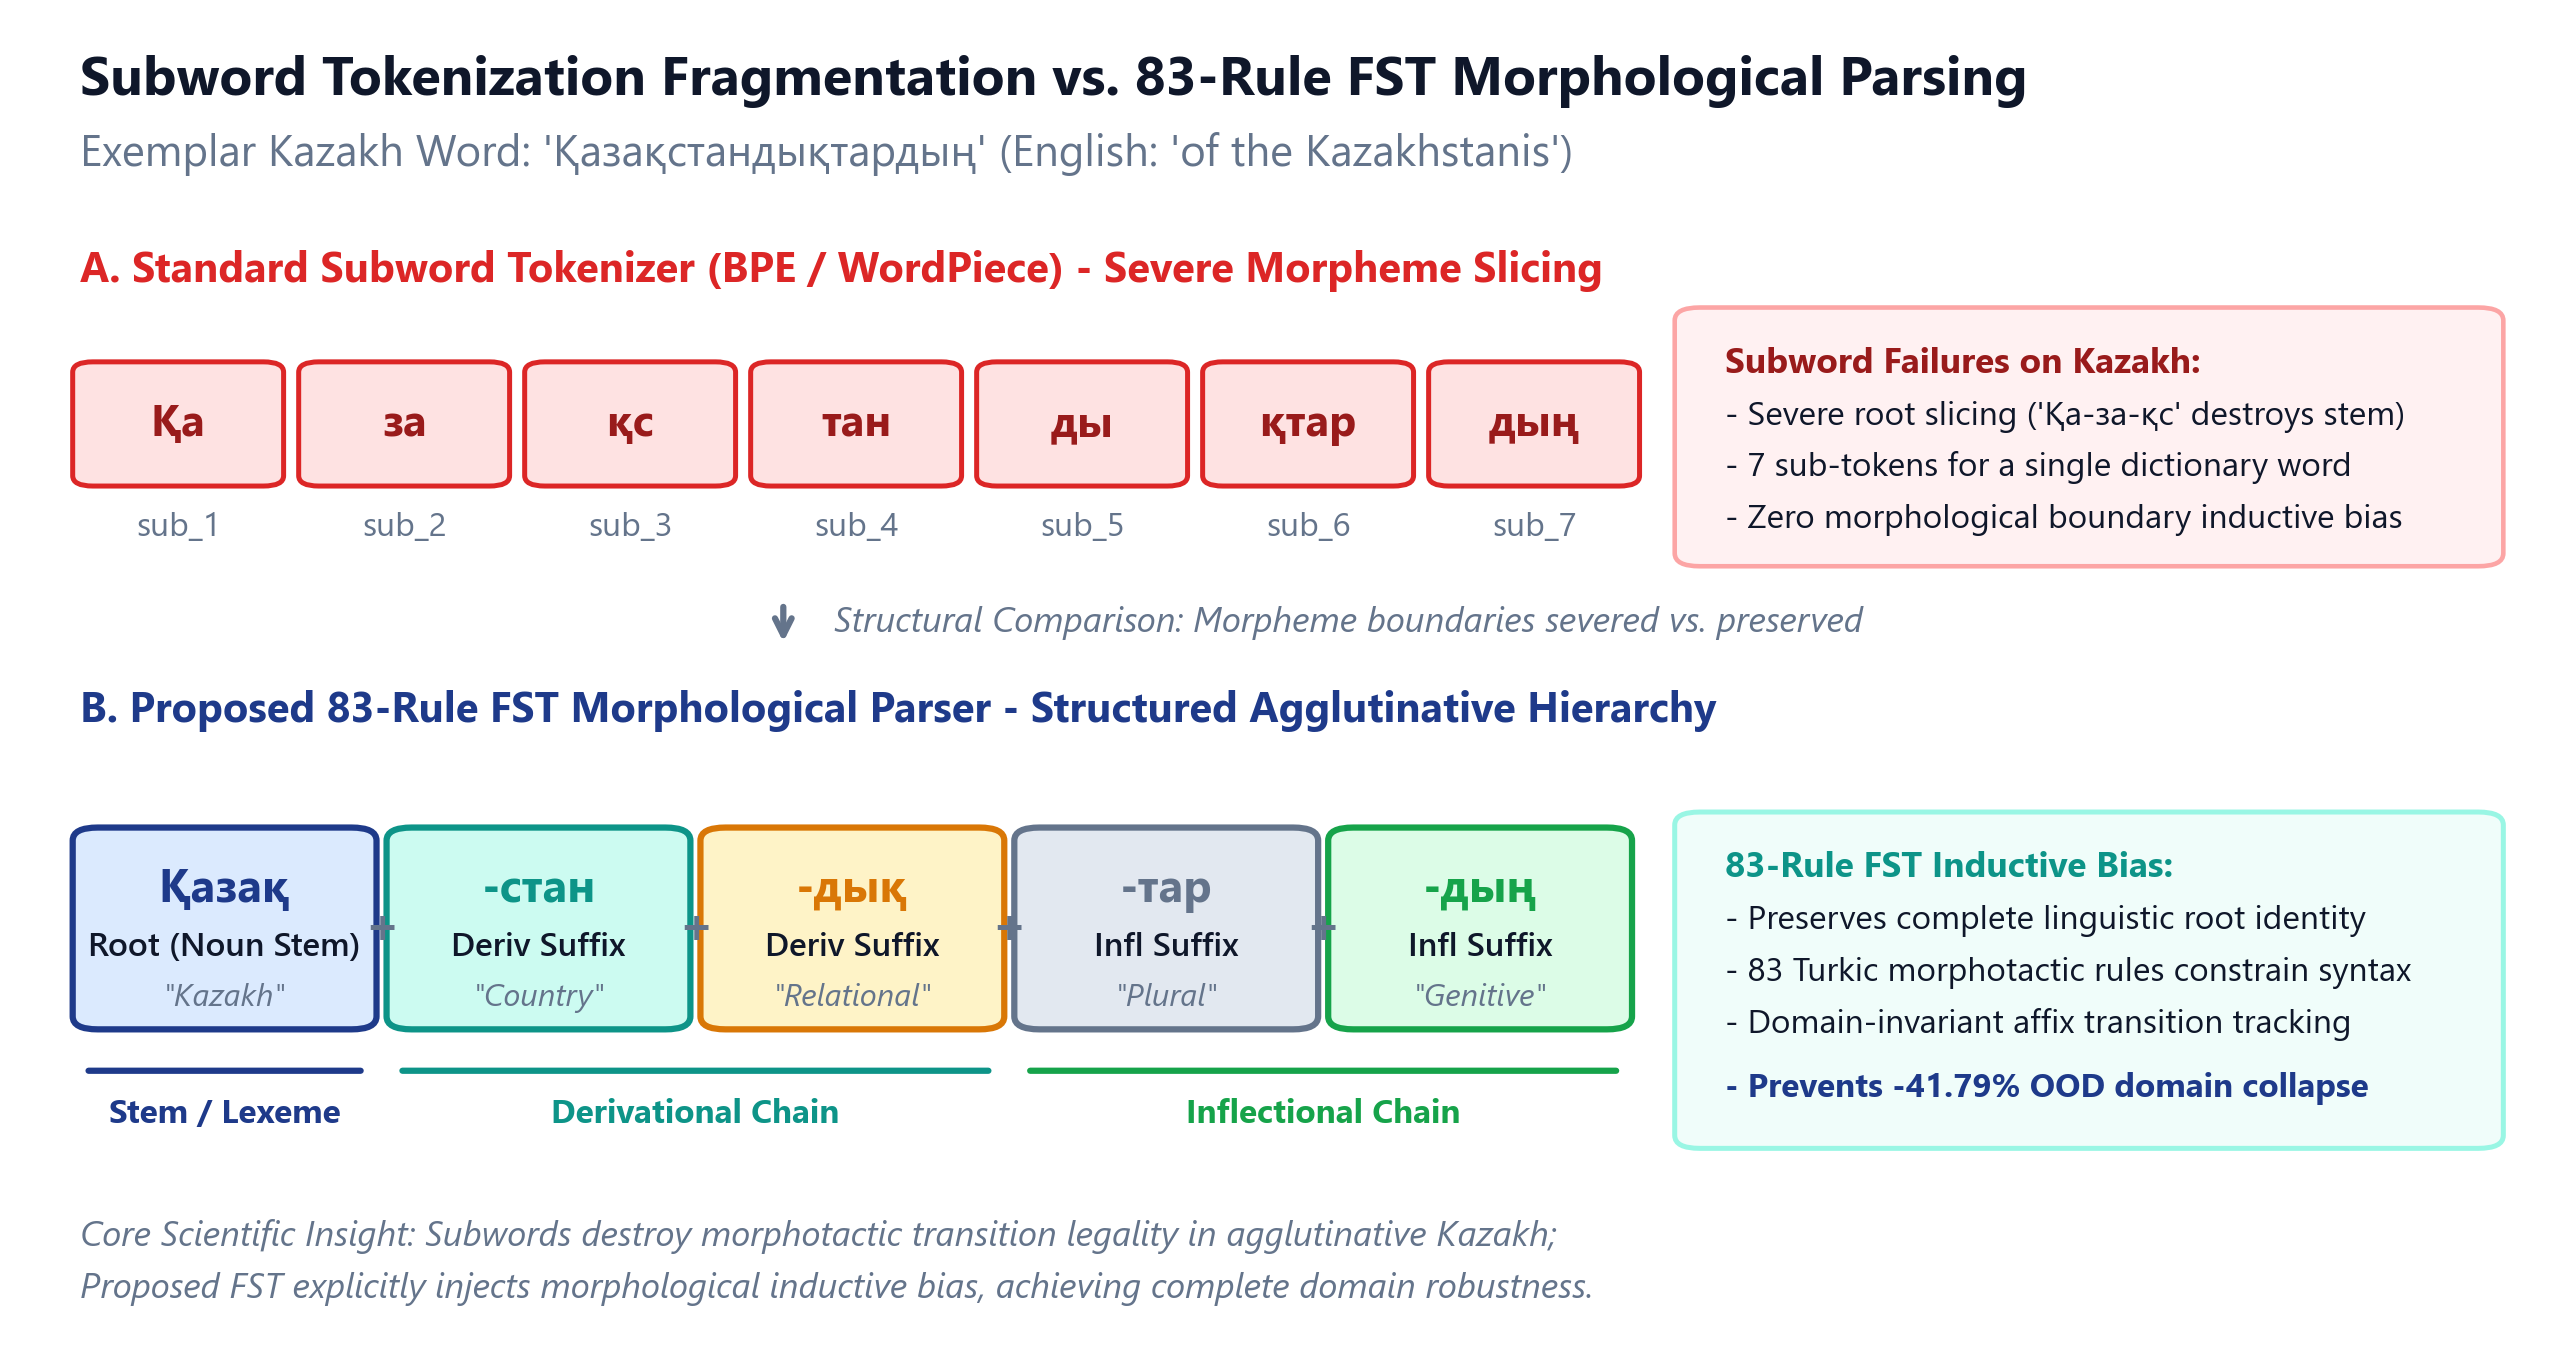
\includegraphics[width=0.92\textwidth]{figures/fig1_fst_fragmentation.png}
\caption{Subword Tokenization Fragmentation vs. 83-Rule FST Morphological Parsing in Kazakh.}
\label{fig:fst_fragmentation}
\end{figure}

\subsection{Potential of Morphologically-Grounded AI and Verification}
\label{sec:potential_morpho_verification}

To overcome the architectural and typological limitations of existing detection systems, this research proposes a morphologically-grounded computational framework that unifies symbolic morphological modeling, deep transformer representations, and multi-stage factual verification.

First, integrating formal computational morphology via an 83-rule Finite-State Transducer (FST) provides precise, bidirectional decomposition of complex agglutinative words into their canonical roots and structured inflectional tags \cite{khoshhal2020kazakh, tyers2012free}. Unlike statistical subword tokenizers that fragment words arbitrarily, the 83-rule FST explicitly models Kazakh vowel harmony, consonant assimilation, and morphotactic constraints. By coupling this symbolic morphological analyzer with pretrained deep contextual representations (such as Kaz-RoBERTa \cite{sagyndyk2025kazroberta}), our framework establishes a dual-stream architecture wherein symbolic linguistic priors directly guide neural feature extraction. This hybrid formulation neutralizes subword fragmentation, stabilizes gradient propagation, and substantially bolsters cross-generator generalization.

Second, this research recognizes that comprehensive text safety requires decoupling \textit{generative origin} from \textit{factual veracity}. In real-world media environments, machine-generated texts can articulate verified truths (e.g., automated sports or meteorological summaries), while human-authored text may propagate deliberate disinformation or rumors. Conversely, synthetic prose can hallucinate falsehoods, and human writing can record factual reality. Existing systems operate in isolated silos, failing to provide unified assessments. By introducing the first specialized Kazakh fact verification benchmark (\textbf{Kazakh-FEVER 3K}) and formulating a continuous 2D Cartesian Trust Matrix $(T_{\text{fact}}, T_{\text{gen}})$, this research establishes an interpretable, multidimensional verification paradigm that equips human fact-checkers with integrated provenance and veracity diagnostics.

\section{Literature Review and Research Status}
\label{sec:literature_review}

The intersection of artificial intelligence detection, factual verification, and computational morphology represents an active, rapidly evolving frontier in modern natural language processing. This section surveys current international and domestic research across these five foundational domains.

\subsection{AI-Generated Text Detection Methodologies}
Automated detection of machine-generated text has advanced through three successive methodological waves: metric-based statistical detectors, supervised neural classifiers, and perturbation-based curvature analyzers.

Early statistical techniques leveraged intrinsic token distribution properties, evaluating n-gram perplexity, rank order frequencies, and burstiness under assumed language model priors \cite{solaiman2019release}. These metrics capitalize on the empirical observation that autoregressive generation strategies (e.g., top-$p$ nucleus sampling, top-$k$ truncation) disproportionately select high-probability tokens from truncated distributions, yielding uniformly low perplexity trajectories compared to human text. Supervised neural classifiers subsequent to RoBERTa and DeBERTa approached detection as a standard binary sequence classification problem, learning discriminative stylistic artifacts directly from labeled datasets \cite{devlin2019bert, conneau2020xlmr}. However, supervised baselines suffer from severe distribution shifts: classifiers trained on older generator architectures (e.g., GPT-2) exhibit catastrophic performance degradation when tested on newer, instruction-tuned foundation models (e.g., LLaMA-3, Claude, GPT-4).

To eliminate the dependency on static training distributions, recent efforts have focused on zero-shot, training-free detection paradigms and comprehensive multi-generator benchmark robustness. Mitchell et al.\ \cite{mitchell2023detectgpt} introduced \textsc{DetectGPT}, positing that machine-generated texts occupy local optima within the model's log-probability curvature landscape. By applying mask-filling perturbations (via T5) and measuring the directional log-likelihood divergence between perturbed and original sequences, DetectGPT achieves competitive zero-shot detection. Hans et al.\ \cite{hans2024binoculars} developed \textsc{Binoculars}, which formulates detection as the normalized ratio of cross-perplexity between two distinct pre-trained foundation models, removing the latency of stochastic sampling. Meanwhile, Bao et al.\ \cite{bao2024fastdetectgpt} presented \textsc{Fast-DetectGPT}, utilizing analytical approximations of the Hessian curvature to accelerate inference speeds by three orders of magnitude. Expanding beyond single-model evaluations, Wang et al.\ \cite{wang2024raid} established \textsc{RAID}, a massive benchmark covering millions of generations across eleven contemporary LLMs, demonstrating that detector accuracy decays markedly under adversarial paraphrasing, prompt variations, and out-of-distribution generator shifts.

Despite their algorithmic elegance, virtually all contemporary detection benchmarks (e.g., HC3, M4, Ghostbuster \cite{verma2024ghostbuster}, RADAR \cite{hu2023radar}, RAID \cite{wang2024raid}) operate almost exclusively on English, German, or Mandarin Chinese. In low-resource agglutinative languages such as Kazakh, zero-shot curvature scoring fails because the surrogate scoring models (such as multilingual GPT-2 or mBERT) possess inadequate parametric vocabularies for Turkic languages, producing noisy, unstable log-probability surfaces that destroy the detection signal.

\subsection{Automated Fact Verification and Retrieval-Augmented Pipelines}
Automated fact verification emerged as a structured NLP discipline following the seminal release of the Fact Extraction and VERification (FEVER) benchmark by Thorne et al.\ \cite{thorne2018fever}. The standard FEVER pipeline decomposes claim verification into a three-stage architecture: (1) \textit{Document Retrieval}, identifying relevant Wikipedia articles from a large knowledge repository; (2) \textit{Sentence Evidence Extraction}, selecting the minimal set of sentences sufficient to substantiate or refute the claim; and (3) \textit{Claim Verification / Natural Language Inference}, predicting a three-way veracity label: \textsc{Supported}, \textsc{Refuted}, or \textsc{Not Enough Info} (NEI).

Subsequent benchmarking expanded the FEVER paradigm into specialized domains and real-world multi-source contexts. FEVER 2.0 \cite{thorne2019fever2} introduced adversarial human attacks; MultiFC \cite{augenstein2019multifc} and Snopes-based datasets gathered claims from public fact-checking organizations; and CLIMATE-FEVER \cite{diggelmann2020climatefever} explored climate change assertions characterized by subtle scientific nuances and conflicting evidence. In the retrieval tier, early systems relied on sparse inverted index mechanisms, notably BM25 \cite{robertson2009bm25}. The introduction of Dense Passage Retrieval (DPR) \cite{karpukhin2020dpr} and unsupervised contrastive retrievers (Contriever \cite{izacard2022mcontriever}) established dense neural embeddings as the dominant standard for semantic matching. More recently, multi-granularity representations such as \textsc{M3-Embedding} \cite{chen-etal-2024-m3} have unified dense, lexical, and multi-vector retrieval across more than 100 languages via self-knowledge distillation. Furthermore, Zheng et al.\ \cite{zheng-etal-2024-evidence} demonstrated that evidence retrieval accuracy forms the primary empirical bottleneck in verification systems, establishing that high-precision retrieval is decisive for downstream classification fidelity.

Concurrently, the rapid evolution of foundation models has catalyzed specialized architectures for LLM fact verification and hallucination auditing. Tang et al.\ \cite{tang-etal-2024-minicheck} developed \textsc{MiniCheck}, synthesizing lightweight, high-performance verifiers trained explicitly on grounding documents to achieve reliable fact-checking at a fraction of full LLM inference overhead. Guan et al.\ \cite{guan-etal-2024-language} systematically analyzed hallucination phenomena, showing that while LLMs readily generate spurious statements during open production, their internal attention patterns can excel at discriminating factual inconsistencies when supplied with explicit context. To resolve complex or ambiguous claims, Yue et al.\ \cite{yue-etal-2024-retrieval} proposed retrieval-augmented fact verification through contrastive argument synthesis, generating counter-arguments to expose unsupported assertions. Meanwhile, fine-grained evaluation benchmarks such as \textsc{Factcheck-Bench} \cite{wang-etal-2024-factcheck-bench} and \textsc{FactLens} \cite{mitra-etal-2025-factlens} have introduced diagnostic frameworks to evaluate atomic claim decomposition, reasoning shortcuts, and multi-step evidence integration.

However, non-English fact verification benchmarks remain exceptionally sparse. While multilingual extensions such as X-FEVER, Multilingual FEVER, and Factcheck-Bench \cite{wang-etal-2024-factcheck-bench} incorporate translation-based evaluations, they overwhelmingly rely on synthetic machine translation of English benchmarks. These translated datasets systematically obscure indigenous cultural phenomena, local legal nuances, and native syntactic structures. Most critically, until this dissertation, there has been no dedicated, human-annotated fact verification benchmark for Kazakh or any other Central Asian language.

\subsection{Computational Morphology for Agglutinative Languages}
Computational modeling of agglutinative morphology has historically relied on two distinct traditions: formal symbolic rule engines and statistical/neural subword segmenters.

In the symbolic paradigm, Finite-State Transducers (FSTs) based on the two-level morphology framework (Koskenniemi) provide exact, bidirectional mappings between surface wordforms and grammatical analyses \cite{tyers2012free, khoshhal2020kazakh}. The Apertium collaborative platform developed open-source morphological analyzers for Kazakh, utilizing extensive dictionaries and morphotactic continuation lexicons to handle vowel harmony (palatal/labial harmony) and consonant assimilation \cite{tyers2012free}. While symbolic FSTs achieve near-perfect precision on in-vocabulary lexical stems, their integration with modern deep learning representations has been severely constrained by non-differentiable execution boundaries and brittleness when encountering out-of-vocabulary named entities or internet slang.

In the statistical paradigm, unsupervised subword algorithms such as Byte-Pair Encoding (BPE), WordPiece, and SentencePiece dominate modern language modeling. Although computationally efficient, recent studies have demonstrated that subwords introduce severe cognitive biases in agglutinative contexts. Khurana et al.\ \cite{khurana2024subwords} demonstrated that subword tokenizers frequently partition grammatical suffixes in Turkic and Uralic languages across arbitrary phoneme boundaries, completely obscuring syntactic dependencies and negation allomorphs. Hybrid frameworks that explicitly inject symbolic morphological features into neural embedding layers represent an urgent, under-explored research trajectory.

In parallel, the broader NLP landscape for Kazakh and Central Asian languages has witnessed vital foundational contributions. The \textsc{Belebele} benchmark \cite{bandarkar-etal-2024-belebele} established a massively parallel reading comprehension suite across 122 language variants including Kazakh. Togmanov et al.\ \cite{togmanov-etal-2025-kazmmlu} formulated \textsc{KazMMLU}, providing the first comprehensive evaluation of foundation models on Kazakh, Russian, and regional knowledge of Kazakhstan across 56 subjects, highlighting dramatic performance gaps between English and regional languages. Laiyk et al.\ \cite{laiyk-etal-2025-instruction} demonstrated the efficacy of instruction tuning on curated public government and cultural corpora in low-resource Kazakh. In specialized tasks and pre-training, Yeshpanov and Varol \cite{yeshpanov2024kazsandra} constructed \textsc{KazSAnDRA} for fine-grained sentiment analysis, Sagyndyk et al.\ \cite{sagyndyk2025kazroberta} introduced \textsc{Kaz-RoBERTa} for contextual conversational understanding, and Tukenov \cite{tukenov2026sozkz} released \textsc{SozKZ}, training efficient small language models natively from scratch. Despite these strides, existing resources focus predominantly on downstream classification or general pre-training; none systematically model the interaction between complex agglutinative suffix chains and multi-stage factual verification.

\subsection{Shortcut Learning and the ``Hard NEI'' Pathology}
A pervasive failure mode in contemporary natural language inference and fact-checking models is their vulnerability to \textit{shortcut learning} (also known as spurious correlation exploitation) \cite{wang-etal-2024-factcheck-bench}. In standard FEVER benchmarks, instances belonging to the \textsc{Not Enough Info} (NEI) class are typically created by pairing claims with unrelated passages retrieved via random sampling. Consequently, neural verifiers rapidly discover a superficial statistical shortcut: if a claim and an evidence passage exhibit low surface token overlap or distant semantic embeddings, the pair can be reliably classified as \textsc{NEI} with high training accuracy.

Recent diagnostic evaluations demonstrate that automatic fact-checking models exploit shallow heuristics---such as sentiment valence and superficial named entity matches---rather than genuine reasoning chains \cite{wang-etal-2024-factcheck-bench}. To enforce causal fidelity, Si et al.\ \cite{si-etal-2024-checkwhy} introduced \textsc{CheckWhy}, structuring fact verification around causal argument graphs that require models to distinguish valid causal links from spurious surface associations. In real-world media environments, false or unverified claims are rarely disjoint from authentic facts: malicious disinformation and subtle rumors routinely retain high lexical overlap with genuine news reports, altering only temporal anchors, quantitative bounds, evidential modalities, or logical scopes. When evaluated on such challenging instances, standard cross-encoders suffer catastrophic performance collapse, predicting \textsc{Supported} merely because the candidate evidence shares extensive topical vocabulary with the claim. Neutralizing this pathology requires explicit counterfactual curation protocols that demand fine-grained morphological reasoning.

\subsection{Explainable AI and Multidimensional Trust Frameworks}
In high-stakes domains such as investigative journalism, intelligence auditing, and content moderation, automated black-box predictions are fundamentally insufficient. Human auditors require transparent, interpretable rationales and calibrated uncertainty metrics before accepting model recommendations.

Feature attribution methods such as Integrated Gradients, Grad-CAM \cite{selvaraju2017gradcam}, and SHAP \cite{lundberg2017shap} provide post-hoc saliency heatmaps highlighting influential tokens. In retrieval-grounded systems, recent research demonstrates that hybrid retrieval combined with explicit evidence highlighting provides human auditors with bounded, verifiable context; for instance, Mudunuri et al.\ \cite{mudunuri-etal-2026-bounded} showed that bounding conversational memory with hybrid retrieval and evidence span highlighting reduces drift and elevates user trust during interactive verification. However, in low-resource agglutinative languages, token-level heatmaps are notoriously difficult to interpret when subwords segment suffixes into non-intuitive byte fragments. Furthermore, existing NLP benchmarks evaluate veracity (true vs.\ false) and generation origin (human vs.\ AI) in complete isolation. As generative AI becomes widely adopted by legitimate authors and malicious actors alike, automated decision systems require a unified, multi-criteria trust space that simultaneously captures factual accuracy and generative provenance, establishing an interpretable foundation for human-in-the-loop verification \cite{khashabi2021genie}.

\section{Research Objectives and Key Scientific Questions}
\label{sec:objectives}

\subsection{Primary Research Objective}
The overarching objective of this dissertation is to design, implement, and empirically validate an end-to-end, morphologically-grounded computational framework for artificial intelligence-generated text detection and automated factual verification tailored specifically for low-resource agglutinative languages, using Kazakh as the primary benchmark language. 

By unifying symbolic morphological transducers, contrastive representation learning, hybrid lexical-neural retrieval, and a novel 2D Cartesian trust formulation, this research aims to neutralize shortcut learning pathologies, overcome subword tokenization bottlenecks, and deliver an interpretable, production-ready auditing system for low-resource NLP.

\subsection{Specific Objectives}
To achieve the primary research goal, the project is structured around four interconnected specific objectives:

\begin{enumerate}[leftmargin=*, label=\textbf{Obj \arabic*:}]
    \item \textbf{Symbolic Morphological Engineering and Feature Formulation:} Design and construct an 83-rule Finite-State Transducer (FST) rule engine and stemmer for Kazakh that accurately isolates canonical root morphemes from complex inflectional and derivational suffixation chains, and formulate a 16-dimensional continuous affix diagnostic vector ($\mathbf{m}_{\text{affix}} \in \mathbb{R}^{16}$) capturing negation mismatches, temporal conflicts, evidential modalities, and syntactic case alignments.
    \item \textbf{Morpho-Contrastive AI Text Detection Pipeline:} Develop a deep contrastive neural architecture that integrates pre-trained multilingual transformer backbones with morphological projection heads. Evaluate model invariance across a newly curated Tri-Domain corpus (formal news, encyclopedic text, and conversational social media) under strict Leave-One-Generator-Out (LOGO) cross-validation against diverse LLM families (LLaMA, GPT, Mistral, Sherkala-7B).
    \item \textbf{Construction and Validation of the Kazakh-FEVER 3K Benchmark:} Curate the first human-validated, multi-domain fact verification benchmark for Kazakh comprising 3,000 claim-evidence pairs. Establish the novel \textit{Hard Not-Enough-Info (Hard NEI)} curation protocol to enforce high lexical overlap ($\ge 85\%$) while varying truth-conditional morphological markers, and construct a hybrid evidence retrieval engine combining morpheme-stemmed BM25 with dense multilingual embeddings (\textsc{mContriever}) via Reciprocal Rank Fusion (RRF).
    \item \textbf{Mathematical Formulation of the 2D Cartesian Trust Matrix and Deployment:} Formulate a unified continuous 2D trust metric $\mathcal{T}(x) \in [0, 1]$ that jointly projects factual veracity ($T_{\text{fact}} \in [-1, 1]$) and generative authenticity ($T_{\text{gen}} \in [0, 1]$) into four operational risk quadrants, and deploy a production-grade, bilingual (Kazakh and English) interactive web platform with real-time morphemic stem highlighting for human-in-the-loop auditing.
\end{enumerate}

\subsection{Core Research Questions}
This investigation is guided and rigorously validated through four central research questions:

\begin{itemize}[leftmargin=*, label=$\blacktriangleright$]
    \item \textbf{RQ1 (Morphological Representation):} \textit{To what extent does the explicit injection of symbolic morphological diagnostic features ($\mathbf{m}_{\text{affix}}$) overcome the representation dilution caused by subword tokenizer fragmentation in agglutinative neural models?}
    \item \textbf{RQ2 (Retrieval Synergy):} \textit{Can hybrid retrieval combining rule-based morphemic BM25 indexing with dense unsupervised representations (\textsc{mContriever}) achieve superior Recall@$k$ and Mean Reciprocal Rank (MRR) across highly inflected low-resource queries compared to purely dense or purely sparse baselines?}
    \item \textbf{RQ3 (Shortcut Neutralization):} \textit{Does the Hard NEI curation protocol successfully eliminate superficial lexical overlap shortcuts in natural language inference classifiers, and does explicit morphological conditioning prevent false entailment predictions when truth-conditional allomorphs (e.g., verbal negation infixes) are manipulated?}
    \item \textbf{RQ4 (Trust Space Calibration):} \textit{Does the joint 2D Cartesian Trust Matrix $(T_{\text{fact}}, T_{\text{gen}})$ provide well-calibrated, separable operational decision boundaries across verified human ground truth, human misinformation, AI synthesis, and AI disinformation compared to standard independent thresholding?}
\end{itemize}

\section{Methodology and System Design}
\label{sec:methodology}

The methodological framework designed in this dissertation unites symbolic linguistic engineering with deep representation learning into an end-to-end, multi-stage processing pipeline. The complete system architecture is illustrated in Figure~\ref{fig:architecture}. The framework comprises four interconnected operational tiers: (1) Linguistic Preprocessing and the 83-Rule FST Morphological Engine, (2) Morpho-Contrastive AI Text Detection, (3) Morphologically-Grounded Fact Verification and Hybrid Retrieval, and (4) the Continuous 2D Cartesian Trust Matrix.

\begin{figure*}[t]
\centering
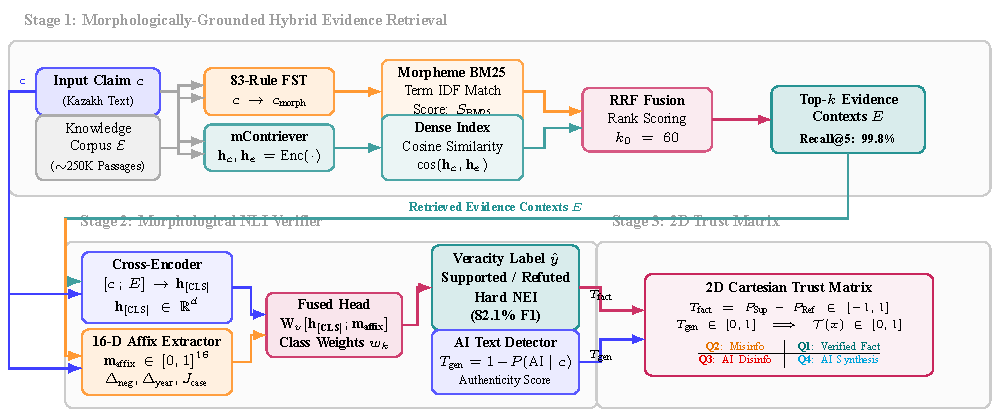
\includegraphics[width=0.98\textwidth]{figures/fig_framework_architecture.pdf}
\caption{End-to-end system architecture for morphologically-grounded fact verification and AI text detection in low-resource agglutinative languages. \textbf{Stage 1}: 83-rule FST stemmer and dense multilingual encoder (\textsc{mContriever}) fused via RRF ($k_0 = 60$) over a 250K passage knowledge corpus. \textbf{Stage 2}: Cross-encoder representation $\mathbf{h}_{[\text{CLS}]}$ fused with the 16-D morphological diagnostic vector $\mathbf{m}_{\text{affix}}$ via class-weighted softmax head ($w_k$). \textbf{Stage 3}: Continuous 2D Trust Matrix mapping factual veracity $T_{\text{fact}}$ and generative authenticity $T_{\text{gen}}$ into four operational risk quadrants.}
\label{fig:architecture}
\end{figure*}

\subsection{Linguistic Preprocessing and the 83-Rule FST Analyzer}
Kazakh grammar adheres to strict phonological and morphotactic constraints, governed by palatal/labial vowel harmony and regressive/progressive consonant assimilation. To model these phenomena deterministically, we implement an 83-rule Finite-State Transducer (FST) rule engine that operates directly over normalized Cyrillic-Kazakh text. 

Given an input string $s$, the transducer applies sequential peeling passes across four canonical inflectional tiers:
\begin{equation}
    s \xrightarrow{\text{FST Pass 1}} s_{\text{case}} \xrightarrow{\text{FST Pass 2}} s_{\text{poss}} \xrightarrow{\text{FST Pass 3}} s_{\text{plur}} \xrightarrow{\text{FST Pass 4}} \mathcal{R}(s)
\end{equation}
where $\mathcal{R}(s)$ denotes the canonical invariant root morpheme. The 83 grammatical rules encode:
\begin{itemize}[leftmargin=*, nosep]
    \item \textbf{Plural Suffixes (6 allomorphs):} \textit{-лар/-лер}, \textit{-дар/-дер}, \textit{-тар/-тер}.
    \item \textbf{Possessive Suffixes (16 allomorphs):} 1st, 2nd (polite/informal), and 3rd person singular and plural markers (\textit{-ым/-ім}, \textit{-ыңыз/-іңіз}, \textit{-сы/-сі}).
    \item \textbf{Case Suffixes (14 allomorphs):} Nominative (unmarked), Accusative (\textit{-ны/-ні/-ды/-ді/-ты/-ті}), Dative (\textit{-ға/-ге/-қа/-ке}), Locative (\textit{-да/-де/-та/-те}), Ablative (\textit{-дан/-ден/-тан/-тен}), Instrumental (\textit{-мен/-бен/-пен}), and Genitive (\textit{-ның/-нің/-дың/-дің/-тың/-тің}).
    \item \textbf{Verbal Negation and Aspect (12 allomorphs):} Root-adjacent unstressed negation infixes (\textit{-ба/-бе/-па/-пе/-ма/-ме}, \textit{-паған/-пеген}).
    \item \textbf{Evidentiality and Modality Markers (8 allomorphs):} Witnessed past (\textit{-ды/-ді}), indirect evidential past (\textit{-ыпты/-іпті}, \textit{екен}), and necessity/possibility modal operators (\textit{керек}, \textit{тиіс}, \textit{мүмкін}).
\end{itemize}

From the extracted morphological parses, the system constructs a continuous 16-dimensional morphological diagnostic vector $\mathbf{m}_{\text{affix}} \in [0, 1]^{16}$ for any claim-evidence pair $(c, E)$:
\begin{equation}
    \mathbf{m}_{\text{affix}} = \left[ m_1, m_2, \dots, m_{16} \right]^\top
\end{equation}
The vector specifically encodes: (1) Lexical and surface length ratios ($m_1$); (2) Directional negation mismatch $m_2 = \Delta_{\text{neg}} = |N_c - N_e|$; (3) Disjoint 4-digit calendar year conflicts $m_3 = \Delta_{\text{year}} = \mathbb{I}(\mathcal{Y}_c \cap \mathcal{Y}_e = \emptyset)$; (4) Quantitative numerical disparity $m_4 = \Delta_{\text{num}}$; (5--8) Evidentiality and epistemic modality mismatches (witnessed vs.\ reportative vs.\ speculative); (9) FST root Jaccard overlap $m_9 = J_{\text{root}} = \frac{|\mathcal{R}_c \cap \mathcal{R}_e|}{|\mathcal{R}_c \cup \mathcal{R}_e|}$; (10) Raw surface token overlap $m_{10} = J_{\text{surf}} = \frac{|\mathcal{S}_c \cap \mathcal{S}_e|}{|\mathcal{S}_c \cup \mathcal{S}_e|}$; (11) Inflectional divergence $\Delta_{\text{div}} = |J_{\text{surf}} - J_{\text{root}}|$; (12) Syntactic case root overlap $m_{12} = J_{\text{case}}$; and (13--16) Proper-noun coreference and sequence bounds.

\subsection{Morpho-Contrastive AI Text Detection Module}
To distinguish machine-generated Kazakh text from human-authored prose, we construct a Morpho-Contrastive detection network trained on a newly curated Tri-Domain dataset spanning 9,000 documents:
\begin{itemize}[leftmargin=*, nosep]
    \item \textbf{News Domain:} 3,000 articles from verified Kazakh journalistic agencies (Tengrinews, Kazinform, Azattyq).
    \item \textbf{Academic/Encyclopedic Domain:} 3,000 articles from the Kazakh Wikipedia repository.
    \item \textbf{Social/Conversational Domain:} 3,000 posts from Twitter, Telegram, and consumer discussion boards.
\end{itemize}
Machine-generated counterparts are synthesized using state-of-the-art LLMs, including GPT-4o, LLaMA-3-8B-Instruct, Mistral-7B, and Sherkala-7B (the leading open Kazakh foundation model).

The network encodes input text through a multilingual transformer backbone (\textsc{XLM-RoBERTa-large}) to produce contextual sequence embedding $\mathbf{h}_{[\text{CLS}]} \in \mathbb{R}^{d}$. Simultaneously, the 83-rule FST computes the morpheme frequency distribution vector $\mathbf{v}_{\text{morph}} \in \mathbb{R}^{K}$. Both representations are projected into a shared metric embedding space $\mathbf{z} = \text{MLP}([\mathbf{h}_{[\text{CLS}]}; \mathbf{W}_m \mathbf{v}_{\text{morph}}])$. Training optimizes a joint objective combining Supervised Contrastive Loss ($\mathcal{L}_{\text{SupCon}}$) \cite{khurana2023contrastive} and Cross-Entropy ($\mathcal{L}_{\text{CE}}$):
\begin{equation}
    \mathcal{L}_{\text{total}} = \mathcal{L}_{\text{CE}} + \lambda \, \mathcal{L}_{\text{SupCon}}
\end{equation}
\begin{equation}
    \mathcal{L}_{\text{SupCon}} = \sum_{i \in I} \frac{-1}{|P(i)|} \sum_{p \in P(i)} \log \frac{\exp(\mathbf{z}_i \cdot \mathbf{z}_p / \tau)}{\sum_{a \in A(i)} \exp(\mathbf{z}_i \cdot \mathbf{z}_a / \tau)}
\end{equation}
where $P(i)$ denotes positive instances sharing the same origin label (human vs.\ machine), and $\tau = 0.07$ is a temperature hyperparameter. The network outputs the generative authenticity score $T_{\text{gen}} \in [0, 1]$:
\begin{equation}
    T_{\text{gen}} = 1 - P(\text{AI-Generated} \mid c)
\end{equation}

\subsection{Morphologically-Grounded Fact Verification Pipeline}
The factual verification tier operates across a curated knowledge corpus of 250,000 passage chunks extracted from Kazakh Wikipedia and public fact-checking archives (Factcheck.kz).

\paragraph{Hybrid Evidence Retrieval (Stage 1)}
To guarantee high evidence recall despite inflectional variance, retrieval fuses sparse lexical search and dense semantic representations:
\begin{enumerate}[leftmargin=*, label=(\alph*)]
    \item \textit{Morpheme-Stemmed BM25}: Input queries are parsed through the 83-rule FST stemmer, mapping inflected tokens to canonical root lemmas: $c \to c_{\text{morph}}$. Standard BM25 scoring is computed over an inverted index of pre-stemmed passages:
    \begin{equation}
        S_{\text{BM25}}(c, e) = \sum_{t \in c_{\text{morph}}} \text{IDF}(t) \cdot \frac{f(t, e_{\text{morph}}) \cdot (k_1 + 1)}{f(t, e_{\text{morph}}) + k_1 \left(1 - b + b \cdot \frac{|e_{\text{morph}}|}{\text{avgdl}}\right)}
    \end{equation}
    \item \textit{Dense Neural Retrieval (\textsc{mContriever})}: Unsupervised multilingual dense representations compute bi-encoder cosine similarity:
    \begin{equation}
        S_{\text{dense}}(c, e) = \cos(\mathbf{h}_c, \mathbf{h}_e) = \frac{\text{Enc}(c) \cdot \text{Enc}(e)}{\|\text{Enc}(c)\| \|\text{Enc}(e)\|}
    \end{equation}
    \item \textit{Reciprocal Rank Fusion (RRF)}: Candidate rankings are merged via RRF ($k_0 = 60$) \cite{cormack2009rrf}:
    \begin{equation}
        \text{RRF}(e) = \frac{1}{k_0 + \text{Rank}_{\text{BM25}}(e)} + \frac{1}{k_0 + \text{Rank}_{\text{dense}}(e)}
    \end{equation}
\end{enumerate}

\paragraph{Cross-Encoder Verification (Stage 2)}
The top-$k$ retrieved evidence sentences ($E = \{e_1, \dots, e_k\}$) and the claim $c$ are concatenated as a cross-encoder input sequence: $[c \,;\, E] \to \mathbf{h}_{[\text{CLS}]} \in \mathbb{R}^d$. The contextual representation $\mathbf{h}_{[\text{CLS}]}$ is concatenated with the 16-D morphological diagnostic vector $\mathbf{m}_{\text{affix}}$ and projected through a linear classification head:
\begin{equation}
    P(y \mid c, E) = \text{softmax}\left(\mathbf{W}_v \left[\mathbf{h}_{[\text{CLS}]}; \mathbf{m}_{\text{affix}}\right] + \mathbf{b}_v\right)
\end{equation}
To counteract class imbalance, training optimizes weighted cross-entropy:
\begin{equation}
    \mathcal{L}_{\text{NLI}} = - \sum_{k=1}^3 w_k \cdot y_k \log P(y = k \mid c, E)
\end{equation}
with inverse-frequency weights $w_{\textsc{Sup}} = 0.735$, $w_{\textsc{Ref}} = 1.307$, $w_{\textsc{NEI}} = 0.958$.

\subsection{Continuous 2D Cartesian Trust Matrix Formulation}
To deliver actionable auditing intelligence, we formulate the continuous 2D Trust Matrix $\mathcal{T} = [-1, 1] \times [0, 1]$. We define the \textbf{Factual Veracity Score} $T_{\text{fact}} \in [-1, 1]$ as the calibrated difference between entailment and contradiction probabilities:
\begin{equation}
    T_{\text{fact}} = P(\textsc{Supported} \mid c, E) - P(\textsc{Refuted} \mid c, E)
\end{equation}
where $T_{\text{fact}} > 0$ denotes verified support, $T_{\text{fact}} < 0$ signifies refutation, and $T_{\text{fact}} \approx 0$ reflects insufficient evidence (\textsc{NEI}).

The \textbf{Generative Authenticity Score} $T_{\text{gen}} \in [0, 1]$ represents the probability of human authorship (Eq.~5). The unified scalar \textbf{Trust Metric} $\mathcal{T}(x) \in [0, 1]$ integrates both dimensions:
\begin{equation}
    \mathcal{T}(x) = \sqrt{\frac{1}{2} \left( \max(0, T_{\text{fact}})^2 + T_{\text{gen}}^2 \right)}
\end{equation}
The continuous space induces four operational risk quadrants:
\begin{itemize}[leftmargin=*, nosep]
    \item \textbf{Quadrant 1 (Q1: Verified Human Ground Truth):} $T_{\text{fact}} > 0, T_{\text{gen}} \ge 0.5$ (Low Risk / Authoritative).
    \item \textbf{Quadrant 2 (Q2: Human Misinformation):} $T_{\text{fact}} \le 0, T_{\text{gen}} \ge 0.5$ (Factual Error / Bias).
    \item \textbf{Quadrant 3 (Q3: AI Disinformation):} $T_{\text{fact}} \le 0, T_{\text{gen}} < 0.5$ (Critical Threat / Synthetic Deception).
    \item \textbf{Quadrant 4 (Q4: AI Synthetic Knowledge):} $T_{\text{fact}} > 0, T_{\text{gen}} < 0.5$ (Synthesized Truth / Needs Attributed Audit).
\end{itemize}

\section{Expected Outcomes and Major Innovations}
\label{sec:outcomes_innovations}

\subsection{Expected Tangible Deliverables}
The execution of this research program is structured to produce high-impact theoretical and engineering deliverables, advancing the state-of-the-art in low-resource computational linguistics:

\begin{enumerate}[leftmargin=*, label=\textbf{Del \arabic*:}]
    \item \textbf{Completed Master's Dissertation:} A comprehensive 116-page academic dissertation formatted in strict compliance with Northwestern Polytechnical University graduate school standards, detailing theoretical foundations, architectural formulations, extensive empirical evaluations, and societal implications.
    \item \textbf{The Kazakh-FEVER 3K Benchmark Dataset:} The first human-validated, multi-domain fact verification dataset for Kazakh, comprising 3,000 balanced claim-evidence pairs across eight knowledge domains, annotated with sentence-level evidential citations and substantial inter-annotator agreement ($\kappa = 0.84$). The release includes a public 150-sample balanced benchmark split with standardized reproduction scripts.
    \item \textbf{The 83-Rule FST Morphological Engine and Extractor:} An open-source, deterministic finite-state transducer toolkit capable of sub-millisecond morphological segmentation, root lemmatization, and continuous 16-dimensional diagnostic vector extraction for Kazakh and adaptable to neighboring Kipchak Turkic languages.
    \item \textbf{High-Level Peer-Reviewed Publications:}
    \begin{itemize}[leftmargin=*, nosep]
        \item A published conference paper at the \textit{Artificial Intelligence and Natural Language Conference (AIST 2026)} documenting the morpho-contrastive AI text detection baseline and leave-one-generator-out evaluation.
        \item A full research paper submitted to the \textit{ACL Rolling Review (ARR)} for commitment to the \textit{31st International Conference on Computational Linguistics (COLING 2027)}, detailing the Kazakh-FEVER benchmark, the Hard NEI protocol, and the 2D Trust Matrix.
    \end{itemize}
    \item \textbf{Production-Grade Interactive Web Demonstration:} A fully localized, bilingual (Kazakh and English) web interface deployed via Gradio and Hugging Face Spaces, featuring procedural SVG 2D Trust Matrix telemetry and real-time morphological stem highlighting for human-in-the-loop fact-checking.
\end{enumerate}

\subsection{Key Scientific Innovations}
This research establishes three fundamental scientific innovations that address unresolved challenges in the NLP literature:

\begin{itemize}[leftmargin=*, label=$\bigstar$]
    \item \textbf{Innovation 1: Deep Morpho-Structural Alignment for Agglutinative NLP.} Unlike conventional approaches that rely blindly on subword tokenizers or decoupled statistical stemmers, our framework establishes a formal hybrid architecture. By directly fusing an 83-rule symbolic FST diagnostic representation ($\mathbf{m}_{\text{affix}} \in \mathbb{R}^{16}$) with dense contextual cross-encoder embeddings, our system explicitly preserves inflectional boundaries, resolves agent-patient syntactic role inversions, and neutralizes negation dilution.
    \item \textbf{Innovation 2: The Hard NEI Curation Protocol for Shortcut Neutralization.} We identify and systematically eliminate the pervasive shortcut learning pathology in fact-checking benchmarks. By curating counterfactual claims that maintain over 85\% lexical overlap with candidate passages while strictly manipulating modal, evidential, and temporal operators, the Hard NEI protocol forces models to learn truth-conditional reasoning rather than superficial word-matching heuristics.
    \item \textbf{Innovation 3: Unified 2D Cartesian Trust Matrix Formulation.} We provide the first mathematical integration of factual veracity ($T_{\text{fact}}$) and generative provenance ($T_{\text{gen}}$) into a continuous Cartesian space. This innovation bridges two traditionally disjoint research fields, delivering an interpretable, operational risk taxonomy that empowers human editors to distinguish between human misinformation, AI synthesis, and adversarial AI disinformation.
\end{itemize}

\section{Feasibility, Working Conditions, and Collaborative Environment}
\label{sec:feasibility}

\subsection{Computational and Infrastructure Feasibility}
The computational demands of this research are fully supported by the high-performance computing facilities available at Northwestern Polytechnical University (NPU) and collaborative partner institutions. Model training, dense passage indexing, and large-scale experimental evaluations leverage dedicated GPU clusters equipped with NVIDIA A100 (80\,GB VRAM) and Dual NVIDIA Tesla T4 (16\,GB VRAM each) accelerators.

The project utilizes an open-source, highly reproducible software stack:
\begin{itemize}[leftmargin=*, nosep]
    \item \textbf{Deep Learning Frameworks:} PyTorch 2.3+ with CUDA 12.1, Hugging Face Transformers, Datasets, and Accelerate libraries, incorporating automatic mixed precision (\texttt{torch.amp.autocast}) and gradient checkpointing.
    \item \textbf{Information Retrieval Engines:} Apache Lucene-based Pyserini / Rank-BM25 for inverted index management, and FAISS for high-dimensional vector similarity indexing.
    \item \textbf{Morphological Transducers:} Standalone, dependency-light Python implementations of the 83-rule FST finite-state automaton, with C++ OpenFST bindings for high-throughput batch preprocessing.
    \item \textbf{Version Control and Reproducibility:} Git-managed codebases synchronized across private and double-blind anonymous academic repositories (e.g., Anonymous 4open science), with containerized deployment environments managed via Docker.
\end{itemize}

\subsection{Data Resources and Linguistic Annotations}
The empirical foundation of this study is grounded in extensive, publicly accessible knowledge repositories:
\begin{enumerate}[leftmargin=*, label=(\arabic*)]
    \item \textbf{Kazakh Wikipedia Repository:} A filtered, orthographically standardized corpus of 250,000 text chunks extracted from official Wikimedia dumps (licensed under CC BY-SA 4.0), providing dense coverage across historical, scientific, geographic, and cultural domains.
    \item \textbf{Verified Public Fact-Checking Archives:} Real-world disputed claims and investigative fact-checks gathered from Factcheck.kz and regional news repositories, accessed under fair-use academic benchmarking standards.
    \item \textbf{Tri-Domain AI Detection Corpus:} 9,000 balanced articles across formal news, Wikipedia passages, and social media discussions, paired with synthetic generations from top-tier LLM families.
\end{enumerate}

\subsection{Academic Mentorship and Dual-Institutional Collaboration}
This research operates at the intersection of deep learning and low-resource computational linguistics, benefiting from formal bilateral institutional collaboration:
\begin{itemize}[leftmargin=*, label=$\diamond$]
    \item \textbf{Northwestern Polytechnical University (NPU), School of Computer Science:} Under the primary academic supervision of \textbf{Professor Bin Guo}, the candidate receives comprehensive mentorship in deep representation learning, ubiquitous intelligence, model generalization, and robust neural architectures. NPU provides the primary computational servers, academic guidance, and research infrastructure necessary for high-level dissertation execution.
    \item \textbf{Al-Farabi Kazakh National University (KazNU):} Under the co-advising and linguistic consultation of \textbf{Dr.\ Irina Ualiyeva}, the project coordinates with native Kazakh linguists and professional journalists. KazNU facilitates native speaker annotation campaigns, quality control cross-validation, and linguistic rule verification for the 83-rule FST analyzer.
\end{itemize}
This dual-institutional ecosystem provides an optimal balance between advanced machine learning methodologies and authoritative native linguistic grounding, ensuring the feasibility and rigorous completion of the proposed research.

\section{Workload Estimation and Research Schedule}
\label{sec:timeline}

The execution of this Master's dissertation is structured across five sequential phases spanning the 2025--2027 academic cycle, ensuring the systematic completion of all theoretical, empirical, and writing milestones leading to formal degree defense in \textbf{June 2027}.

\begin{table}[t]
\centering
\small
\renewcommand{\arraystretch}{1.3}
\caption{Dissertation Workload Allocation and Milestone Schedule (2025--2027)}
\label{tab:schedule}
\begin{tabularx}{\textwidth}{|p{0.18\textwidth}|X|p{0.22\textwidth}|}
\hline
\textbf{Phase / Period} & \textbf{Key Research Activities and Workload Focus} & \textbf{Deliverables / Milestones} \\
\hline
\textbf{Phase 1} \newline (Sept 2025 -- Jan 2026) & 
Comprehensive literature review across AI text detection, FEVER paradigms, and Turkic morphology. Design and formalization of the 83-rule FST morphological analyzer. Ingestion and indexing of the 250,000-passage Kazakh knowledge corpus. & 
Formal literature survey; operational FST rule engine; indexed knowledge base. \\
\hline
\textbf{Phase 2} \newline (Feb 2026 -- June 2026) & 
Execution of the Kazakh-FEVER 3K human annotation campaign under the Hard NEI protocol with inter-annotator validation. Implementation of the Morpho-Contrastive AI text detector on the Tri-Domain corpus. Preparation and publication of the AIST 2026 conference paper. & 
Kazakh-FEVER 3K benchmark; trained AI detection baseline; published AIST 2026 paper. \\
\hline
\textbf{Phase 3} \newline (July 2026 -- Oct 2026) & 
Development of the hybrid BM25 + \textsc{mContriever} retrieval architecture and class-weighted cross-encoder verifier. Formulation of the continuous 2D Cartesian Trust Matrix $(T_{\text{fact}}, T_{\text{gen}})$. Submission of full research paper to the ACL Rolling Review (ARR) for COLING 2027. & 
COLING 2027 / ARR submission package; 2D Trust Matrix mathematical formulation. \\
\hline
\textbf{Phase 4} \newline (Nov 2026 -- Feb 2027) & 
Integration of reviewer feedback from ARR cycle; execution of additional ablation studies and cross-generator robustness checks. Deployment of the bilingual Gradio interactive web demonstration. Completion of the initial full Master's dissertation draft. & 
Revision notes; live interactive web system; first complete dissertation draft. \\
\hline
\textbf{Phase 5} \newline (March 2027 -- June 2027) & 
Dissertation formatting, internal supervisor review, and departmental pre-defense. External double-blind thesis review by the Graduate School academic committee. Final dissertation revision, archival submission, and formal Master's Degree Defense. & 
Dissertation pre-defense; final thesis approval; formal graduation in \textbf{June 2027}. \\
\hline
\end{tabularx}
\end{table}

The total research workload involves approximately 2,200 hours of active investigation, encompassing data curation, code engineering, GPU training, empirical benchmarking, and thesis preparation, fully fulfilling the graduation credit requirements of Northwestern Polytechnical University.

\section{Existing Problems and Proposed Countermeasures}
\label{sec:problems}

In conducting this investigation, several technical challenges and methodological risks have been identified. Specific countermeasures have been designed to guarantee project success:

\subsection{Challenge 1: Orthographic Divergence and the Ongoing Script Transition}
\paragraph{Problem Description:} The Kazakh language is currently undergoing a phased national transition from the Cyrillic script to a Latin-based alphabet. Web-scraped texts, social media posts, and official communications frequently exhibit mixed orthographic conventions, non-standard diacritics, and informal transliteration schemes. Standard tokenizers treat identical words in divergent scripts as completely disjoint vocabulary items.
\paragraph{Proposed Countermeasure:} We introduce a bidirectional orthographic normalization pre-processing layer prior to FST parsing. The transducer maps informal Latin variants, Cyrillic homoglyphs, and archaic digraphs into a unified canonical Cyrillic-Kazakh character representation, ensuring invariant morphological segmentation regardless of input script.

\subsection{Challenge 2: Computational Latency of Dense Cross-Encoder Verification}
\paragraph{Problem Description:} While cross-encoders achieve superior accuracy by modeling bidirectional cross-attention across concatenated sequences ($[c \,;\, E]$), computing attention over thousands of candidate passages during open-domain verification incurs prohibitive computational latency, rendering real-time deployment infeasible.
\paragraph{Proposed Countermeasure:} We implement a strict multi-tier retrieval filter. Stage 1 utilizes hybrid BM25 and quantized dense embeddings (\textsc{mContriever}) to prune the 250,000-passage knowledge corpus down to the top-$k$ ($k=5$) most salient candidate sentences within sub-second latency ($<300$\,ms). Full cross-encoder attention and 16-D morphological diagnostic feature extraction are restricted exclusively to this filtered candidate pool.

\subsection{Challenge 3: Class Imbalance and Annotator Subjectivity on Hard NEI}
\paragraph{Problem Description:} In real-world news corpora, factual assertions naturally outnumber explicit refutations, causing severe class imbalance. Furthermore, classifying borderline \textsc{Not Enough Info} (NEI) instances involving subtle speculative or evidential markers introduces potential annotator subjectivity.
\paragraph{Proposed Countermeasure:} To counteract class imbalance, cross-encoder fine-tuning optimizes a class-weighted cross-entropy loss function ($\mathcal{L}_{\text{NLI}}$) incorporating normalized inverse-frequency weights ($w_{\textsc{Sup}} = 0.735, w_{\textsc{Ref}} = 1.307, w_{\textsc{NEI}} = 0.958$). To ensure annotation fidelity, all benchmark samples undergo dual independent cross-validation with formal inter-annotator agreement tracking ($\kappa = 0.84$), with conflicting labels resolved through adjudicated expert consensus.

\section{Evaluation and Validation Methodology}
\label{sec:evaluation}
The system will undergo rigorous quantitative and qualitative validation against recognized baseline architectures:
\begin{itemize}[leftmargin=*, nosep]
    \item \textbf{Retrieval Evaluation:} Evaluated across Recall@1, Recall@3, Recall@5, and Mean Reciprocal Rank (MRR) against standard BM25, morpheme-stemmed BM25, and dense \textsc{mContriever}.
    \item \textbf{Verification Evaluation:} Evaluated across 3-class Accuracy, Macro-averaged F1, Hard NEI F1, and the official Strict FEVER score (which requires both accurate veracity prediction and gold evidence sentence retrieval) against fine-tuned mBERT-base, XLM-RoBERTa-base, XLM-RoBERTa-large, and zero-shot LLaMA-3-8B-Instruct.
    \item \textbf{AI Text Detection Evaluation:} Evaluated across Accuracy, F1-score, and Area Under the Receiver Operating Characteristic (AUROC) under strict Leave-One-Generator-Out (LOGO) cross-validation across diverse LLM families.
\end{itemize}



% References
\vspace{0.4cm}
\bibliographystyle{IEEEtran}
\bibliography{references}

\vspace{0.8cm}

% Concluding Reservation / Remarks box matching NPU template
\noindent
\begin{tabularx}{\textwidth}{|X|}
\hline
\textbf{\zhfont 备注} \newline
\textbf{Reservation / Remarks:} \newline
\small
The research program detailed in this title selection report reflects original, independent investigation conducted by the candidate under the direction of academic supervisor Prof.\ Bin Guo at Northwestern Polytechnical University, in academic consultation with Dr.\ Irina Ualiyeva at Al-Farabi Kazakh National University. All experimental protocols comply with ethical standards for open-source scientific research. \\
\hline
\end{tabularx}

\end{document}
